% Framework figure of ECHO for the LNCS version. Drawn at the LNCS text width
% (12.2 cm) and included at scale 1, so label sizes are what the reader sees.
% Content follows echo/model.py:
%   row A  snapshot evolution -> entity states E_t -> structural intensity
%   row B  dyad streams of the support set -> stream encoder -> candidate
%          state (stream state, 8 statistics, context, entity/query vectors)
%          -> attention across candidates -> dyadic intensity
%   row C  popularity field -> popularity intensity; path propagation from the
%          refined candidate states -> path intensity
%   right  the four intensities are added (log-sum-exp) and entities ranked
\documentclass[border=1pt]{standalone}
\usepackage[T1]{fontenc}
\usepackage[scaled=0.92]{helvet}
\renewcommand{\familydefault}{\sfdefault}
\usepackage{amsmath,amssymb}
\usepackage{tikz}
\usetikzlibrary{arrows.meta,positioning,calc}
\DeclareMathSizes{6.5}{6.5}{5}{5}
\DeclareMathSizes{7.5}{7.5}{5.5}{5}
\newcommand{\lbl}{\fontsize{6.5}{7.6}\selectfont}
\newcommand{\ttlf}{\fontsize{7.5}{8.6}\selectfont\bfseries}
\definecolor{cDyad}{HTML}{2A6F97}
\definecolor{cPath}{HTML}{E07A1F}
\definecolor{cStruct}{HTML}{4C9A2A}
\definecolor{cPop}{HTML}{8E6BBF}
\definecolor{cComp}{HTML}{C0392B}
\definecolor{cGrey}{HTML}{6B6B6B}
\definecolor{rA}{HTML}{1F77B4}\definecolor{rB}{HTML}{2CA02C}\definecolor{rC}{HTML}{D62728}
\definecolor{cO}{HTML}{C0392B}\definecolor{cP}{HTML}{E07A1F}\definecolor{cX}{HTML}{8E6BBF}
\begin{document}
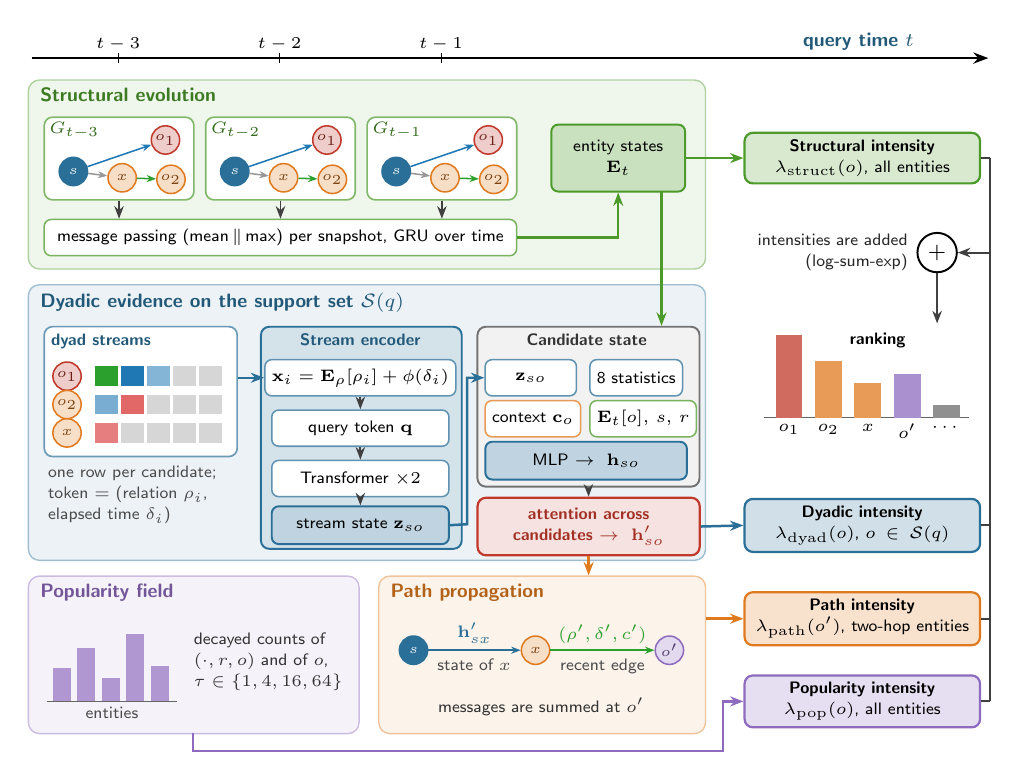
\begin{tikzpicture}[
  x=1cm, y=1cm, font=\lbl,
  panel/.style={fill=#1!9, draw=#1!45, rounded corners=4pt, line width=0.5pt},
  ttl/.style={font=\ttlf, text=#1!80!black, anchor=north west, inner sep=1.5pt},
  card/.style={fill=white, draw=#1!70, rounded corners=3pt, line width=0.6pt},
  pill/.style={fill=white, draw=#1!75, rounded corners=2.5pt, line width=0.55pt, minimum height=4.6mm, inner xsep=2.5pt, inner ysep=1.5pt, align=center},
  key/.style={fill=#1!30, draw=#1, rounded corners=2.5pt, line width=0.7pt, minimum height=4.8mm, inner xsep=2.5pt, inner ysep=1.5pt, align=center},
  outb/.style={fill=#1!22, draw=#1, rounded corners=3pt, line width=0.8pt, inner xsep=2pt, inner ysep=2.5pt, align=center, text width=28.5mm},
  ent/.style={circle, draw=#1, fill=#1!25, minimum size=3.6mm, inner sep=0pt, font=\fontsize{5.5}{6}\selectfont\bfseries, text=#1!55!black, line width=0.55pt},
  sub/.style={ent=cDyad, fill=cDyad, text=white},
  edg/.style={-{Stealth[length=1.2mm]}, line width=0.55pt, #1},
  arr/.style={-{Stealth[length=1.6mm]}, line width=0.7pt, black!75},
  carr/.style={-{Stealth[length=1.7mm]}, line width=0.9pt, #1},
  cell/.style={draw=white, line width=0.35pt},
]
\newcommand{\tokrow}[3]{\foreach \c [count=\i from 0] in {#3} {\fill[\c, cell] (#1+\i*0.33, #2) rectangle ++(0.3,0.26);}}

% ───────────── timeline ─────────────
\draw[-{Stealth[length=1.9mm]}, line width=0.8pt] (0.05,0.32) -- (12.2,0.32);
\foreach \x/\l in {1.15/$t-3$, 3.2/$t-2$, 5.25/$t-1$} {\node[anchor=south, inner sep=2pt] at (\x,0.34) {\l}; \draw (\x,0.26) -- (\x,0.38);}
\node[font=\ttlf, anchor=south, inner sep=2pt, text=cDyad!80!black] at (10.55,0.34) {query time $t$};

% ═════════════ row A: structural evolution ═════════════
\node[panel=cStruct, minimum width=86mm, minimum height=24mm, anchor=north west] (PA) at (0,0.05) {};
\node[ttl=cStruct] at (0.1,0.0) {Structural evolution};
\foreach \x/\k/\tl in {0.2/1/t-3, 2.25/2/t-2, 4.3/3/t-1} {
  \node[card=cStruct, minimum width=19mm, minimum height=10.5mm, anchor=north west] (C\k) at (\x,-0.42) {};
  \node[anchor=north west, inner sep=1.5pt, text=cStruct!70!black] at (\x+0.02,-0.43) {$G_{\tl}$};
  \node[sub] (s\k) at (\x+0.38,-1.12) {$s$};
  \node[ent=cO] (o\k) at (\x+1.55,-0.72) {$o_1$};
  \node[ent=cP] (x\k) at (\x+1.0,-1.2) {$x$};
  \node[ent=cP] (p\k) at (\x+1.62,-1.22) {$o_2$};
  \draw[edg=rA] (s\k) -- (o\k); \draw[edg=cGrey!70] (s\k) -- (x\k); \draw[edg=rB] (x\k) -- (p\k);
}
\node[pill=cStruct, minimum width=60mm, anchor=north west] (mp) at (0.2,-1.72) {message passing (mean\,$\|$\,max) per snapshot, GRU over time};
\foreach \k in {1,2,3} {\draw[arr] (C\k.south) -- (C\k.south |- mp.north);}
\node[key=cStruct, minimum width=17mm, minimum height=8.5mm] (Et) at (7.5,-0.95) {entity states\\$\mathbf{E}_t$};
\draw[carr=cStruct] (mp.east) -| (Et.south);

% ═════════════ row B: dyadic evidence ═════════════
\node[panel=cDyad, minimum width=86mm, minimum height=35mm, anchor=north west] (PB) at (0,-2.55) {};
\node[ttl=cDyad] at (0.1,-2.6) {Dyadic evidence on the support set $\mathcal{S}(q)$};
% B1: dyad streams
\node[card=cDyad, minimum width=24.5mm, minimum height=16.5mm, anchor=north west] (DS) at (0.2,-3.08) {};
\node[anchor=north west, inner sep=2pt, text=cDyad!80!black, font=\lbl\bfseries] at (0.22,-3.1) {dyad streams};
\node[ent=cO] at (0.5,-3.72) {$o_1$};  \tokrow{0.85}{-3.85}{rB,rA,rA!55,cGrey!28,cGrey!28}
\node[ent=cP] at (0.5,-4.08) {$o_2$};  \tokrow{0.85}{-4.21}{rA!60,rC!70,cGrey!28,cGrey!28,cGrey!28}
\node[ent=cP] at (0.5,-4.44) {$x$};    \tokrow{0.85}{-4.57}{rC!60,cGrey!28,cGrey!28,cGrey!28,cGrey!28}
\node[anchor=north west, inner sep=1.5pt, text=black!70, text width=24.5mm, align=left] at (0.2,-4.8) {one row per candidate;\\token $=$ (relation $\rho_i$,\\elapsed time $\delta_i$)};
% B2: stream encoder
\node[fill=cDyad!20, draw=cDyad, rounded corners=3pt, line width=0.7pt, minimum width=25.5mm, minimum height=28.2mm, anchor=north west] (SE) at (2.95,-3.08) {};
\node[font=\lbl\bfseries, text=cDyad!80!black, anchor=north, inner sep=2pt] at (4.225,-3.1) {Stream encoder};
\node[pill=cDyad, minimum width=22.5mm, anchor=north] (tok) at (4.225,-3.5) {$\mathbf{x}_i = \mathbf{E}_\rho[\rho_i] + \phi(\delta_i)$};
\node[pill=cDyad, minimum width=22.5mm, anchor=north] (qt) at (4.225,-4.14) {query token $\mathbf{q}$};
\node[pill=cDyad, minimum width=22.5mm, anchor=north] (trf) at (4.225,-4.78) {Transformer $\times 2$};
\node[key=cDyad, minimum width=22.5mm, anchor=north] (zo) at (4.225,-5.36) {stream state $\mathbf{z}_{so}$};
\draw[arr] (tok) -- (qt); \draw[arr] (qt) -- (trf); \draw[arr] (trf) -- (zo);
\draw[carr=cDyad] (DS.east |- tok.west) -- (tok.west);
% B3: candidate state and attention across candidates
\node[fill=black!5, draw=black!55, rounded corners=3pt, line width=0.7pt, minimum width=28.2mm, minimum height=20.3mm, anchor=north west] (CS) at (5.7,-3.08) {};
\node[font=\lbl\bfseries, text=black!80, anchor=north, inner sep=2pt] at (7.1,-3.1) {Candidate state};
\node[pill=cDyad, minimum width=11.6mm, anchor=north west] (i1) at (5.8,-3.5) {$\mathbf{z}_{so}$};
\node[pill=cDyad, minimum width=11.6mm, anchor=north west] (i2) at (7.13,-3.5) {8 statistics};
\node[pill=cPath, minimum width=11.6mm, anchor=north west] (i3) at (5.8,-4.02) {context $\mathbf{c}_o$};
\node[pill=cStruct, minimum width=11.6mm, anchor=north west] (i4) at (7.13,-4.02) {$\mathbf{E}_t[o],\,s,\,r$};
\node[key=cDyad, minimum width=25.6mm, anchor=north west] (hs) at (5.8,-4.54) {MLP $\rightarrow\ \mathbf{h}_{so}$};
\node[fill=cComp!14, draw=cComp, rounded corners=3pt, line width=0.8pt, minimum width=28.2mm, minimum height=7.3mm, align=center, anchor=north west, font=\lbl\bfseries, text=cComp!85!black] (comp) at (5.7,-5.25) {attention across\\candidates $\rightarrow\ \mathbf{h}'_{so}$};
\draw[arr] (CS.south) -- (comp.north);
\draw[carr=cDyad] (zo.east) -- (5.58,-5.6) |- (i1.west);
\draw[carr=cStruct] (8.05,-1.375) -- (8.05,-3.08);

% ═════════════ row C: popularity and path ═════════════
\node[panel=cPop, minimum width=42mm, minimum height=20mm, anchor=north west] (PP) at (0,-6.25) {};
\node[ttl=cPop] at (0.1,-6.3) {Popularity field};
\foreach \i/\h in {0/0.42, 1/0.68, 2/0.3, 3/0.85, 4/0.45} {\fill[cPop!70] (0.32+\i*0.31,-7.85) rectangle ++(0.23,\h);}
\draw[black!60] (0.24,-7.85) -- (1.9,-7.85);
\node[anchor=north, inner sep=1.5pt, text=black!70] at (1.07,-7.86) {entities};
\node[anchor=west, inner sep=1.5pt, text=black!80, text width=20mm, align=left] at (2.05,-7.35) {decayed counts of $(\cdot, r, o)$ and of $o$,\\$\tau \in \{1, 4, 16, 64\}$};

\node[panel=cPath, minimum width=41.5mm, minimum height=20mm, anchor=north west] (PT) at (4.45,-6.25) {};
\node[ttl=cPath] at (4.55,-6.3) {Path propagation};
\node[sub] (ps) at (4.9,-7.2) {$s$}; \node[ent=cP] (px) at (6.45,-7.2) {$x$}; \node[ent=cX] (po) at (8.15,-7.2) {$o'$};
\draw[edg=cDyad, line width=0.9pt] (ps) -- node[above, inner sep=2pt] {$\mathbf{h}'_{sx}$} (px);
\draw[edg=rB, line width=0.9pt] (px) -- node[above, inner sep=2pt] {$(\rho', \delta', c')$} (po);
\node[anchor=north, inner sep=2.5pt, text=black!70] at (5.67,-7.22) {state of $x$};
\node[anchor=north, inner sep=2.5pt, text=black!70] at (7.3,-7.22) {recent edge};
\node[anchor=north, inner sep=1.5pt, text=black!80] at (6.52,-7.75) {messages are summed at $o'$};
\draw[carr=cPath] (comp.south) -- (comp.south |- PT.north);

% ═════════════ right column: intensities, sum, ranking ═════════════
\node[outb=cStruct] (ls) at (10.6,-0.95) {\textbf{Structural intensity}\\$\lambda_{\mathrm{struct}}(o)$, all entities};
\node[outb=cDyad] (ld) at (10.6,-5.615) {\textbf{Dyadic intensity}\\$\lambda_{\mathrm{dyad}}(o)$, $o \in \mathcal{S}(q)$};
\node[outb=cPath] (lp) at (10.6,-6.8) {\textbf{Path intensity}\\$\lambda_{\mathrm{path}}(o')$, two-hop entities};
\node[outb=cPop] (lpop) at (10.6,-7.85) {\textbf{Popularity intensity}\\$\lambda_{\mathrm{pop}}(o)$, all entities};
\draw[carr=cStruct] (Et.east) -- (ls.west);
\draw[carr=cDyad] (comp.east) -- (ld.west);
\draw[carr=cPath] (PT.east |- lp.west) -- (lp.west);
\draw[carr=cPop] (2.1,-8.25) -- (2.1,-8.48) -- (8.83,-8.48) |- (lpop.west);
% sum and ranking
\node[circle, draw=black, fill=white, line width=0.7pt, inner sep=0pt, minimum size=5mm, font=\fontsize{8}{9}\selectfont] (sum) at (11.55,-2.15) {$+$};
\node[anchor=east, inner sep=3pt, align=right, text=black!85] at (sum.west) {intensities are added\\(log-sum-exp)};
\foreach \n in {ls, ld, lp, lpop} {\draw[black!75, line width=0.7pt] (\n.east) -- (\n.east -| 12.22,0);}
\draw[black!75, line width=0.7pt] (12.22,-0.95) -- (12.22,-7.85);
\draw[arr] (12.22,-2.15) -- (sum.east);
\begin{scope}[shift={(9.35,-4.25)}]
  \draw[black!60] (0,0) -- (2.6,0);
  \foreach \i/\h/\c/\l in {0/1.05/cO/$o_1$, 1/0.72/cP/$o_2$, 2/0.45/cP/$x$, 3/0.56/cX/$o'$, 4/0.16/cGrey/$\cdots$} {\fill[\c!75] (0.15+\i*0.5,0) rectangle ++(0.34,\h); \node[anchor=north, inner sep=2pt] at (0.32+\i*0.5,0) {\l};}
  \node[anchor=west, inner sep=1pt, font=\lbl\bfseries] at (1.05,0.98) {ranking};
\end{scope}
\draw[arr] (sum.south) -- (11.55,-3.05);
\end{tikzpicture}
\end{document}
